\documentclass{article}

\usepackage{amsmath} % Define various maths environments
\usepackage{amssymb} % Define various maths symbols
\usepackage{geometry} % Adjust the margin, paper size, and etc.
\geometry{a4paper, scale = 0.8}
\usepackage{enumerate} % Provide different style of lists
\usepackage{graphicx} % Insert image of all types
\usepackage{xcolor}
\usepackage{ulem}
\usepackage{pdfpages}
\usepackage{array} % Provide auxiliary farmat for tabular
\usepackage{booktabs} % Create Three-line Table
\usepackage{bm}
\usepackage{cite}
\usepackage{url}
\usepackage{float}
\usepackage{indentfirst}
\usepackage{multirow}
\usepackage[colorlinks,linkcolor=black]{hyperref}
\usepackage{subfigure}

\begin{document}

\vspace*{0.4cm}

\hrulefill %??????draw a horizontal line??????

\thispagestyle{empty} %set empty in footnote

\begin{center}
\begin{large}
\scshape{UM--SJTU Joint Institute \vspace{0.3em} \\ Physics Laboratory \\(Vp241)}
\end{large}

\hrulefill %??????draw a horizontal line??????

\vspace*{7.5cm}
\begin{Large}
\scshape{{Laboratory Report}}
\end{Large}

\vspace{2.5em}

\begin{large}
\scshape{Exercise 3}\\
\vspace{0.5em}
\scshape{Solar Cells: $I-V$ Characteristics}
\end{large}
\end{center}

\vspace{13em}

\begin{table}[h!]
\center
\begin{tabular}{lll}
\textbf{Name: Haoming  Zhu} \hspace*{2em}&
\textbf{ID: 520021910145}\hspace*{2em}
& Group: 1 \\
Partner: Xinkai Wang \hspace*{2em}&
ID: 520021910312\hspace*{2em}
& Group: 1 \\
\end{tabular}
\end{table}

\vspace{-0.4cm}

\begin{center}
\hspace{0.3em} Date: 2021.11.19
\end{center}

\newpage
\tableofcontents
\setcounter{page}{0}
\thispagestyle{empty}
\newpage



		\section{Introduction}
	\subsection{Objective}
The objective of this exercise is to preliminarily study the working principle of a solar cell and its current-voltage ($I-V$) characteristics.

	\subsection{Theoretical Background}
\subsubsection{Solar Cell Structure}
A typical crystalline silicon solar cell consists of n=p homo-junctions, a 10 cm $\times$ 10 cm p-type silicon plate of thickness $500~\mu$m, covered with a heavily doped n-type layer with thickness $0.3~\mu$m. The metallic bars on the n-type layer and the metallic film at the bottom play the role of two electrodes respectively. An anti-reflective film is applied to cover the surface that is exposed to light for reducing energy loss. Figure \ref{fig.solar cell} shows the sketch of a crystalline silicon cell used in this lab.

\begin{figure}[H]
\centering
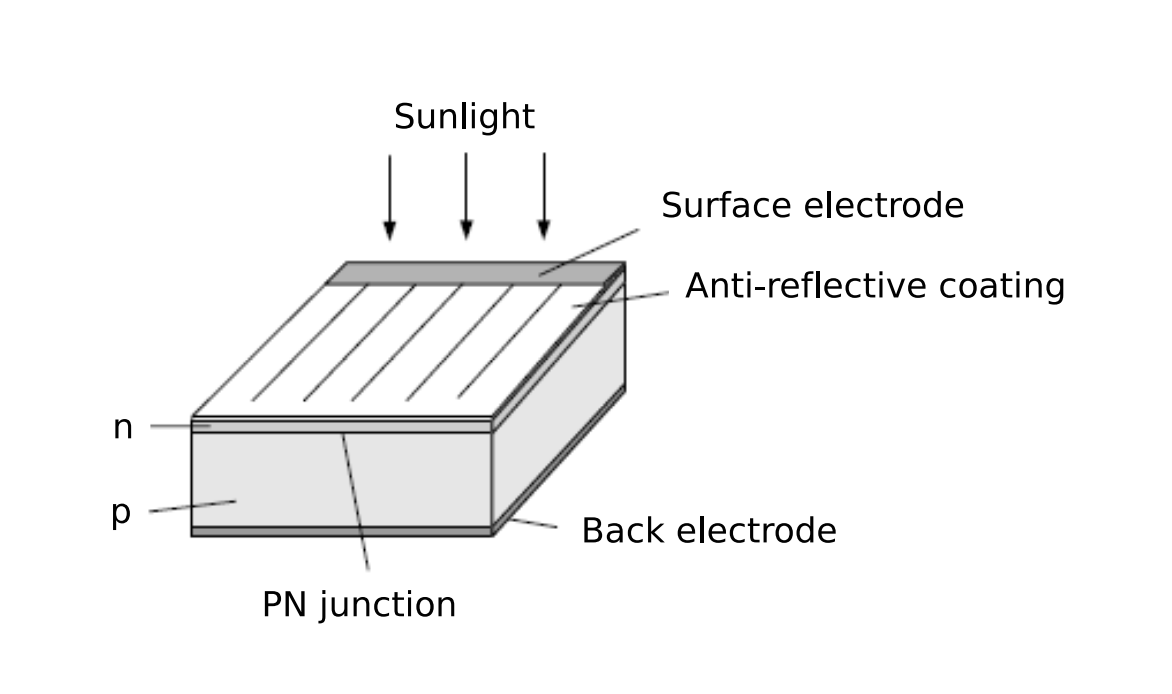
\includegraphics[scale=0.6]{solar cell}
\caption{Structure of a crystalline silicon solar cell.}\label{fig.solar cell}
\end{figure}

\subsubsection{Photovoltaic Effect}
Photovoltaic effect is a phenomenon that when some incident photons with energy greater than the energy gap $E_{\mathrm{g}}$ enter the p-n junction near the solar cell surface, these photons will be absorbed and excite electron-hole pairs. When some charge carriers' energy exceed a certain value, they may diffuse from the n- or p-type area and arrive at the p-n junction, where a built-in electric field (directed from n- to p-type area) exists. Then those minority carries will be drawn by this electric filed to the p-/n-type area in case of holes/electrons. This generates a potential called photoelectric potential.

\subsubsection{Solar Cell Parameters}
Due to the photovoltaic effect, solar cells can generate an electric current $I_{\mathrm{ph}}$ from the n-area to the p-area when there is light incident on the solar cell.

At the same time, in the device there exists a forward diode current $I_{\mathrm{D}}$ from the p-type to the n-type area, opposite to $I_{\mathrm{ph}}$. Eventually, this leads to a net current:

\begin{equation}
I=I_{\mathrm{ph}}-I_{\mathrm{D}}=I_{\mathrm{ph}}-I_{0}\left[\exp \left(\frac{q V_{\mathrm{D}}}{n k_{\mathrm{B}} T}\right)-1\right]
\end{equation}

the quantities in the equation are listed below:

\begin{table}[H]
\centering
\begin{tabular}{ll}
$V_D$ & Junction voltage \\
$I_D$ & Diode inverse saturation current \\
$I_{\mathrm{ph}}$ & Photo-current determined by the structure and material characteristics of the solar cell \\
$n$ & Characteristic theoretical coefficient of p-n Junction, ranging from 1 to 2 \\
$q$ & Electron's charge \\
$k_B$ & Boltzmann's constant \\
$T$ & Temperature in the absolute (Kelvin) scale \\
$R_s$ & Internal series resistance \\
$V$ & Terminal voltage \\
\end{tabular}
\end{table}

Ignoring the internal series resistance $R_s$, the voltage $V_D$ equals the terminal voltage $V$ and \eqref{fig.solar cell} can be rewritten as

\begin{equation}
I=I_{\mathrm{ph}}-I_{0}\left[\exp \left(\frac{q V}{n k_{\mathrm{B}} T}\right)-1\right]
\end{equation}

When the output is short, $i.e. V = 0$, the short circuit current is 

\begin{equation}
I_{\mathrm{sc}} = I_{\mathrm{ph}}
\end{equation} 

whereas when the output is open, i.e. I = 0, the open-circuit voltage is

\begin{equation}
V_{oc} = \frac{nk_{\mathrm{B}}T}{q}ln(\frac{I_{\mathrm{sc}}}{I_{\mathrm{0}}}+1)
\end{equation}

When there is a load resistance $R$ (with the value of $R$ ranging from zero to infinity), the corresponding $I$-$V$ values vary. The figure below shows the relationship between $I$ and $V$.

\begin{figure}[H]
\centering
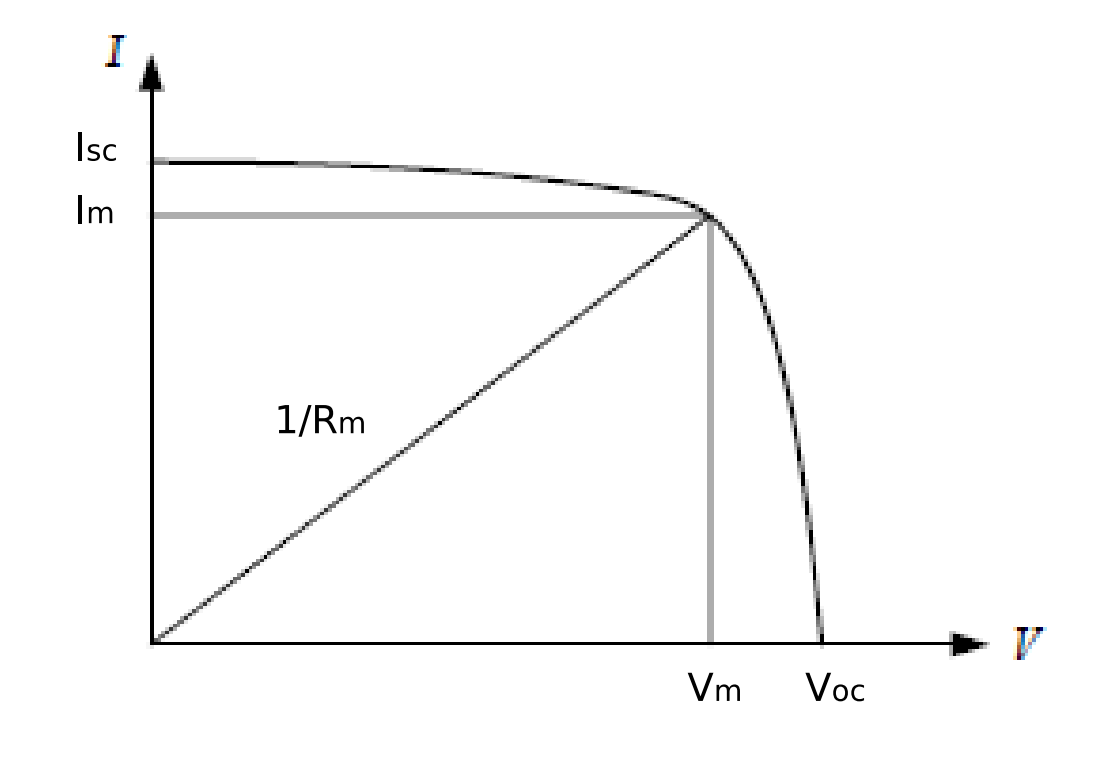
\includegraphics[scale=0.5]{I-V}
\caption{The current-voltage characteristics of a solar cell.}
\end{figure}

If a certain load resistance $R = R_\text{m}$ the maximum output power $P_\text{m}$ is generated, then the value of $P_\text{m}$ is
$$P_\text{m} = I_\text{m}V_\text{m},$$
where $I_\text{m}$ is called the optimal operating current, and $V_\text{m}$ is called the optimal operating voltage.


The $fill factor$ is another important parameter of solar cells, defined as
\begin{equation}
    FF = \frac{P_\text{m}}{V_{\text{oc}}I_{\text{sc}}} = \frac{V_\text{m}I_{\text{m}}}{V_{\text{oc}}I_{\text{sc}}}.
    \label{eq:FF}
\end{equation}
Generally, the greater the fill factor, the greater the output power.

The solar cell energy conversion efficiency $\eta$ is defined as
\begin{equation}
    \eta = \frac{P_\text{m}}{P_{\text{in}}}\times 100\%,
    \label{eq:efficiency}
\end{equation}
where $P_{\text{in}}$ denotes the total radiant power incident on the solar cell.

\subsubsection{Solar Cell Equivalent Circuit}

For convenience, a solar cell can be viewed as composed of p-n junctions diode $D$ and a constant current source $I_{\mathrm{ph}}$. In reality, there will be inner resistance within the cell, therefore the circuit can be viewed as being in series with a resistor $R_{\mathrm{s}}$ and in parallel with a resistor $R_{\mathrm{sh}}$. Combining all these, a p-n junction leak-circuit is formed (Figure \ref{fig.circuit}), with current

\begin{equation}
I=I_{\mathrm{ph}}-I_{0}\left\{\exp \left[\frac{q\left(V+R_{\mathrm{s}} I\right)}{n k_{\mathrm{B}} T}\right]-1\right\}-\frac{V+R_{\mathrm{s}} I}{R_{\mathrm{sh}}}
\end{equation}

\begin{figure}[H]
\centering
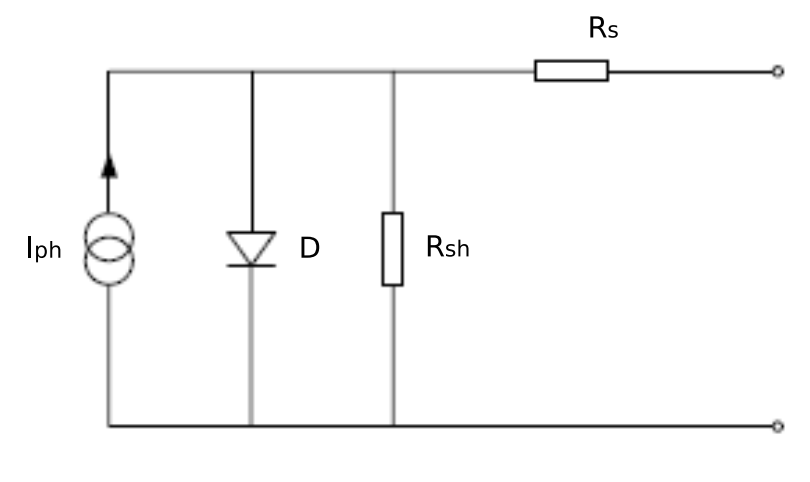
\includegraphics[scale=0.5]{circuit}
\caption{Solar cell equivalent circuit.}\label{fig.circuit}
\end{figure}

		\section{Measurement Setup and Procedure}
The apparatus consists of a photovoltaic device (5 W), a 300 W tungsten{halogen lamp serving as a radiation source, two digital multimeters, two adjustable resistors, a solar power meter, a wiring board and a measuring tape.

The precision of the devices used is shown in Table \ref{tab.precision}.

\begin{table}[H]
    \centering
    \begin{tabular}{cc}
        \toprule
        Quantity    & Uncertainties           \\
        \midrule
        DC voltage  & $\pm~(0.5\% + 0.01)$ [V]  \\
        DC current  & $\pm~(1.5\% + 0.1)$ [mA]  \\
        Distance    & $\pm~0.1$ [cm]            \\
        Solar power & $\pm~10$ [$\text{W/m}^2$] \\
        \bottomrule
    \end{tabular}
    \caption{Precision of the measurement instruments.}\label{tab.precision}
\end{table}

In this experiment, the characteristic of four configurations of the solar cell are studied. For each configuration, $I$-$V$ and $P$-$V$ relations are studied, and for the single configurations, the information about fill factor and energy conversion efficiency are also explored.

The general experiment procedures are summary below:

\begin{enumerate}
\item Turn on both the light and the fan. Wait for at least five minutes, in order to let the light reach its working intensity.
\item Measure the basic parameters of a single panel, including length and width. 
\item In pairs, adjust two panel so that they have same (or very close) $V_{oc}$ and $I_{sc}$. Then use the solar power meter to measure the power of the lights on the two panels.
\item Connect the measurement circuit. Then adjust the resistance so that different data of $V$ and $I$ are obtained. Perform this step for both in series and in parallel configurations.
\item Repeat the measurement procedure for a single device, with the distance maintained the same. Then change the distance and repeat this step.The new distance should be about 80\% or 120\% of the original one.
\end{enumerate}

		\section{Result}
		
	\subsection{$I$-$V$ Relation}
\subsubsection{Series and Parallel Configuration}
	
The measurement results under in series and in parallel configurations are shown in Table \ref{tab.oc-sc} and Table \ref{tab.s-p}.

\begin{table}[H]
\centering
\begin{tabular}{c||c|c|c|c}
\toprule
              & single device at 109.00 cm & single device at 111.21 cm & series & parallel \\ \midrule
$U_{OC}$ {[}V{]}  & 9.12                       & 9.48                       & 18.60  & 9.31     \\ \midrule
$I_{SC}$ {[}mA{]} & 52.5                       & 52.0                       & 52.3   & 104.9    \\ \bottomrule
\end{tabular}\caption{Measurement data for $U_{OC}$ and $I_{SC}$}\label{tab.oc-sc}
\end{table}

\begin{table}[H]
\centering
\begin{tabular}{@{}c|cc||cc@{}}
\toprule
\multirow{2}{*}{} & \multicolumn{2}{c||}{Series} & \multicolumn{2}{c}{Parallel} \\ \midrule
                  & U[V]         & I[mA]       & U[V]         & I[mA]         \\ \midrule
1                 & 0.24         & 52.3        & 9.19         & 9.0           \\
2                 & 0.66         & 52.1        & 9.13         & 12.6          \\
3                 & 0.99         & 51.8        & 9.08         & 15.7          \\
4                 & 1.28         & 51.6        & 9.00         & 20.2          \\
5                 & 2.17         & 51.1        & 8.93         & 24.0          \\
6                 & 3.09         & 50.3        & 8.85         & 28.1          \\
7                 & 4.11         & 49.5        & 8.76         & 32.6          \\
8                 & 5.33         & 48.4        & 8.54         & 41.8          \\
9                 & 6.51         & 47.3        & 8.47         & 44.3          \\
10                & 7.50         & 46.3        & 8.47         & 47.9          \\
11                & 8.26         & 45.7        & 8.26         & 51.7          \\
12                & 9.25         & 44.5        & 8.14         & 55.4          \\
13                & 10.48        & 42.9        & 7.96         & 60.4          \\
14                & 12.02        & 40.8        & 7.81         & 63.6          \\
15                & 13.34        & 38.8        & 7.56         & 68.1          \\
16                & 14.40        & 36.3        & 7.26         & 72.5          \\
17                & 15.18        & 33.5        & 6.66         & 77.8          \\
18                & 16.34        & 26.7        & 5.70         & 84.4          \\
19                & 16.68        & 24.0        & 4.76         & 89.6          \\
20                & 16.96        & 21.5        & 4.02         & 92.8          \\
21                & 17.12        & 20.0        & 2.66         & 97.8          \\
22                & 17.29        & 18.2        & 1.78         & 100.8         \\
23                & 17.37        & 17.5        & 1.00         & 103.7         \\
24                & 17.42        & 17.1        & 0.49         & 105.0         \\
25                & 11.15        & 42.4        & 8.65         & 37.7             \\ \bottomrule
\end{tabular}\caption{Measurement data for the $U$ vs. $I$ relation (series/parallel configuration).} \label{tab.s-p}
\end{table}

\subsubsection{Configurations of Different Distances}

\begin{table}[H]
\centering
\begin{tabular}{c||c|c}
\toprule
              & single device at 109.00 cm & single device at 86.80 cm  \\ \midrule
$U_{OC}$ {[}V{]}  & 9.12                       & 9.48   \\ \midrule
$I_{SC}$ {[}mA{]} & 52.5                      & 68.2  \\ \bottomrule
\end{tabular}\caption{Measurement data for $U_{OC}$ and $I_{SC}$}\label{tab.oc-sc}
\end{table}

\begin{table}[H]
\centering
\begin{tabular}{@{}c|cc||cc@{}}
\toprule
\multirow{2}{*}{} & \multicolumn{2}{c||}{109.00 cm} & \multicolumn{2}{c}{86.80 cm}                \\ \midrule
                  & U[V]              & I[mA]     & U[V]                 & I[mA]                \\ \midrule
1                 & 0.39              & 52.4      & 0.37                 & 68.4                 \\
2                 & 1.70              & 50.0      & 1.66                 & 66.9                 \\
3                 & 2.76              & 48.4      & 2.69                 & 64.7                 \\
4                 & 4.03              & 46.3      & 3.64                 & 62.6                 \\
5                 & \textit{5.00}     & 44.1      & 5.34                 & 59.0                 \\
6                 & 5.52              & 42.3      & 5.52                 & 58.7                 \\
7                 & 6.12              & 39.7      & 6.06                 & 56.6                 \\
8                 & 6.69              & 36.8      & 6.46                 & 54.5                 \\
9                 & 7.15              & 34.1      & 6.95                 & 51.5                 \\
10                & 7.41              & 32.0      & 7.27                 & 49.4                 \\
11                & 7.58              & 30.4      & 7.54                 & 47.5                 \\
12                & 7.77              & 28.3      & 7.79                 & 45.5                 \\
13                & 7.93              & 26.1      & 8.05                 & 42.2                 \\
14                & 8.12              & 23.2      & 8.19                 & 40.1                 \\
15                & 8.25              & 21.0      & 8.33                 & 37.7                 \\
16                & 8.35              & 19.2      & 8.49                 & 34.6                 \\
17                & 8.43              & 17.7      & 8.56                 & 33.0                 \\
18                & 8.55              & 15.1      & 8.66                 & 30.8                 \\
19                & 8.62              & 13.4      & 8.77                 & 28.1                 \\
20                & 8.71              & 11.4      & 8.83                 & 26.3                 \\
21                & 8.75              & 10.4      & 8.89                 & 24.6                 \\
22                & 8.79              & 9.5       & 8.94                 & 23.0                 \\
23                & 8.82              & 8.6       & 8.98                 & 21.7                 \\
24                & 8.39              & 18.3      & 9.32                 & 9.1                  \\
25                & 5.26              & 43.0      & \multicolumn{1}{l}{} & \multicolumn{1}{l}{}  \\ \bottomrule  
\end{tabular}\caption{Measurement data for the $U$ vs. $I$ relation (109.00 cm/86.80 cm configuration).} \label{tab.diff-dist}
\end{table}

The $I-V$ characteristics curves of the four configurations are plotted in Figure \ref{fig.I-U} using \textbf{\textit{Origin}}.

\begin{figure}[H]
\centering
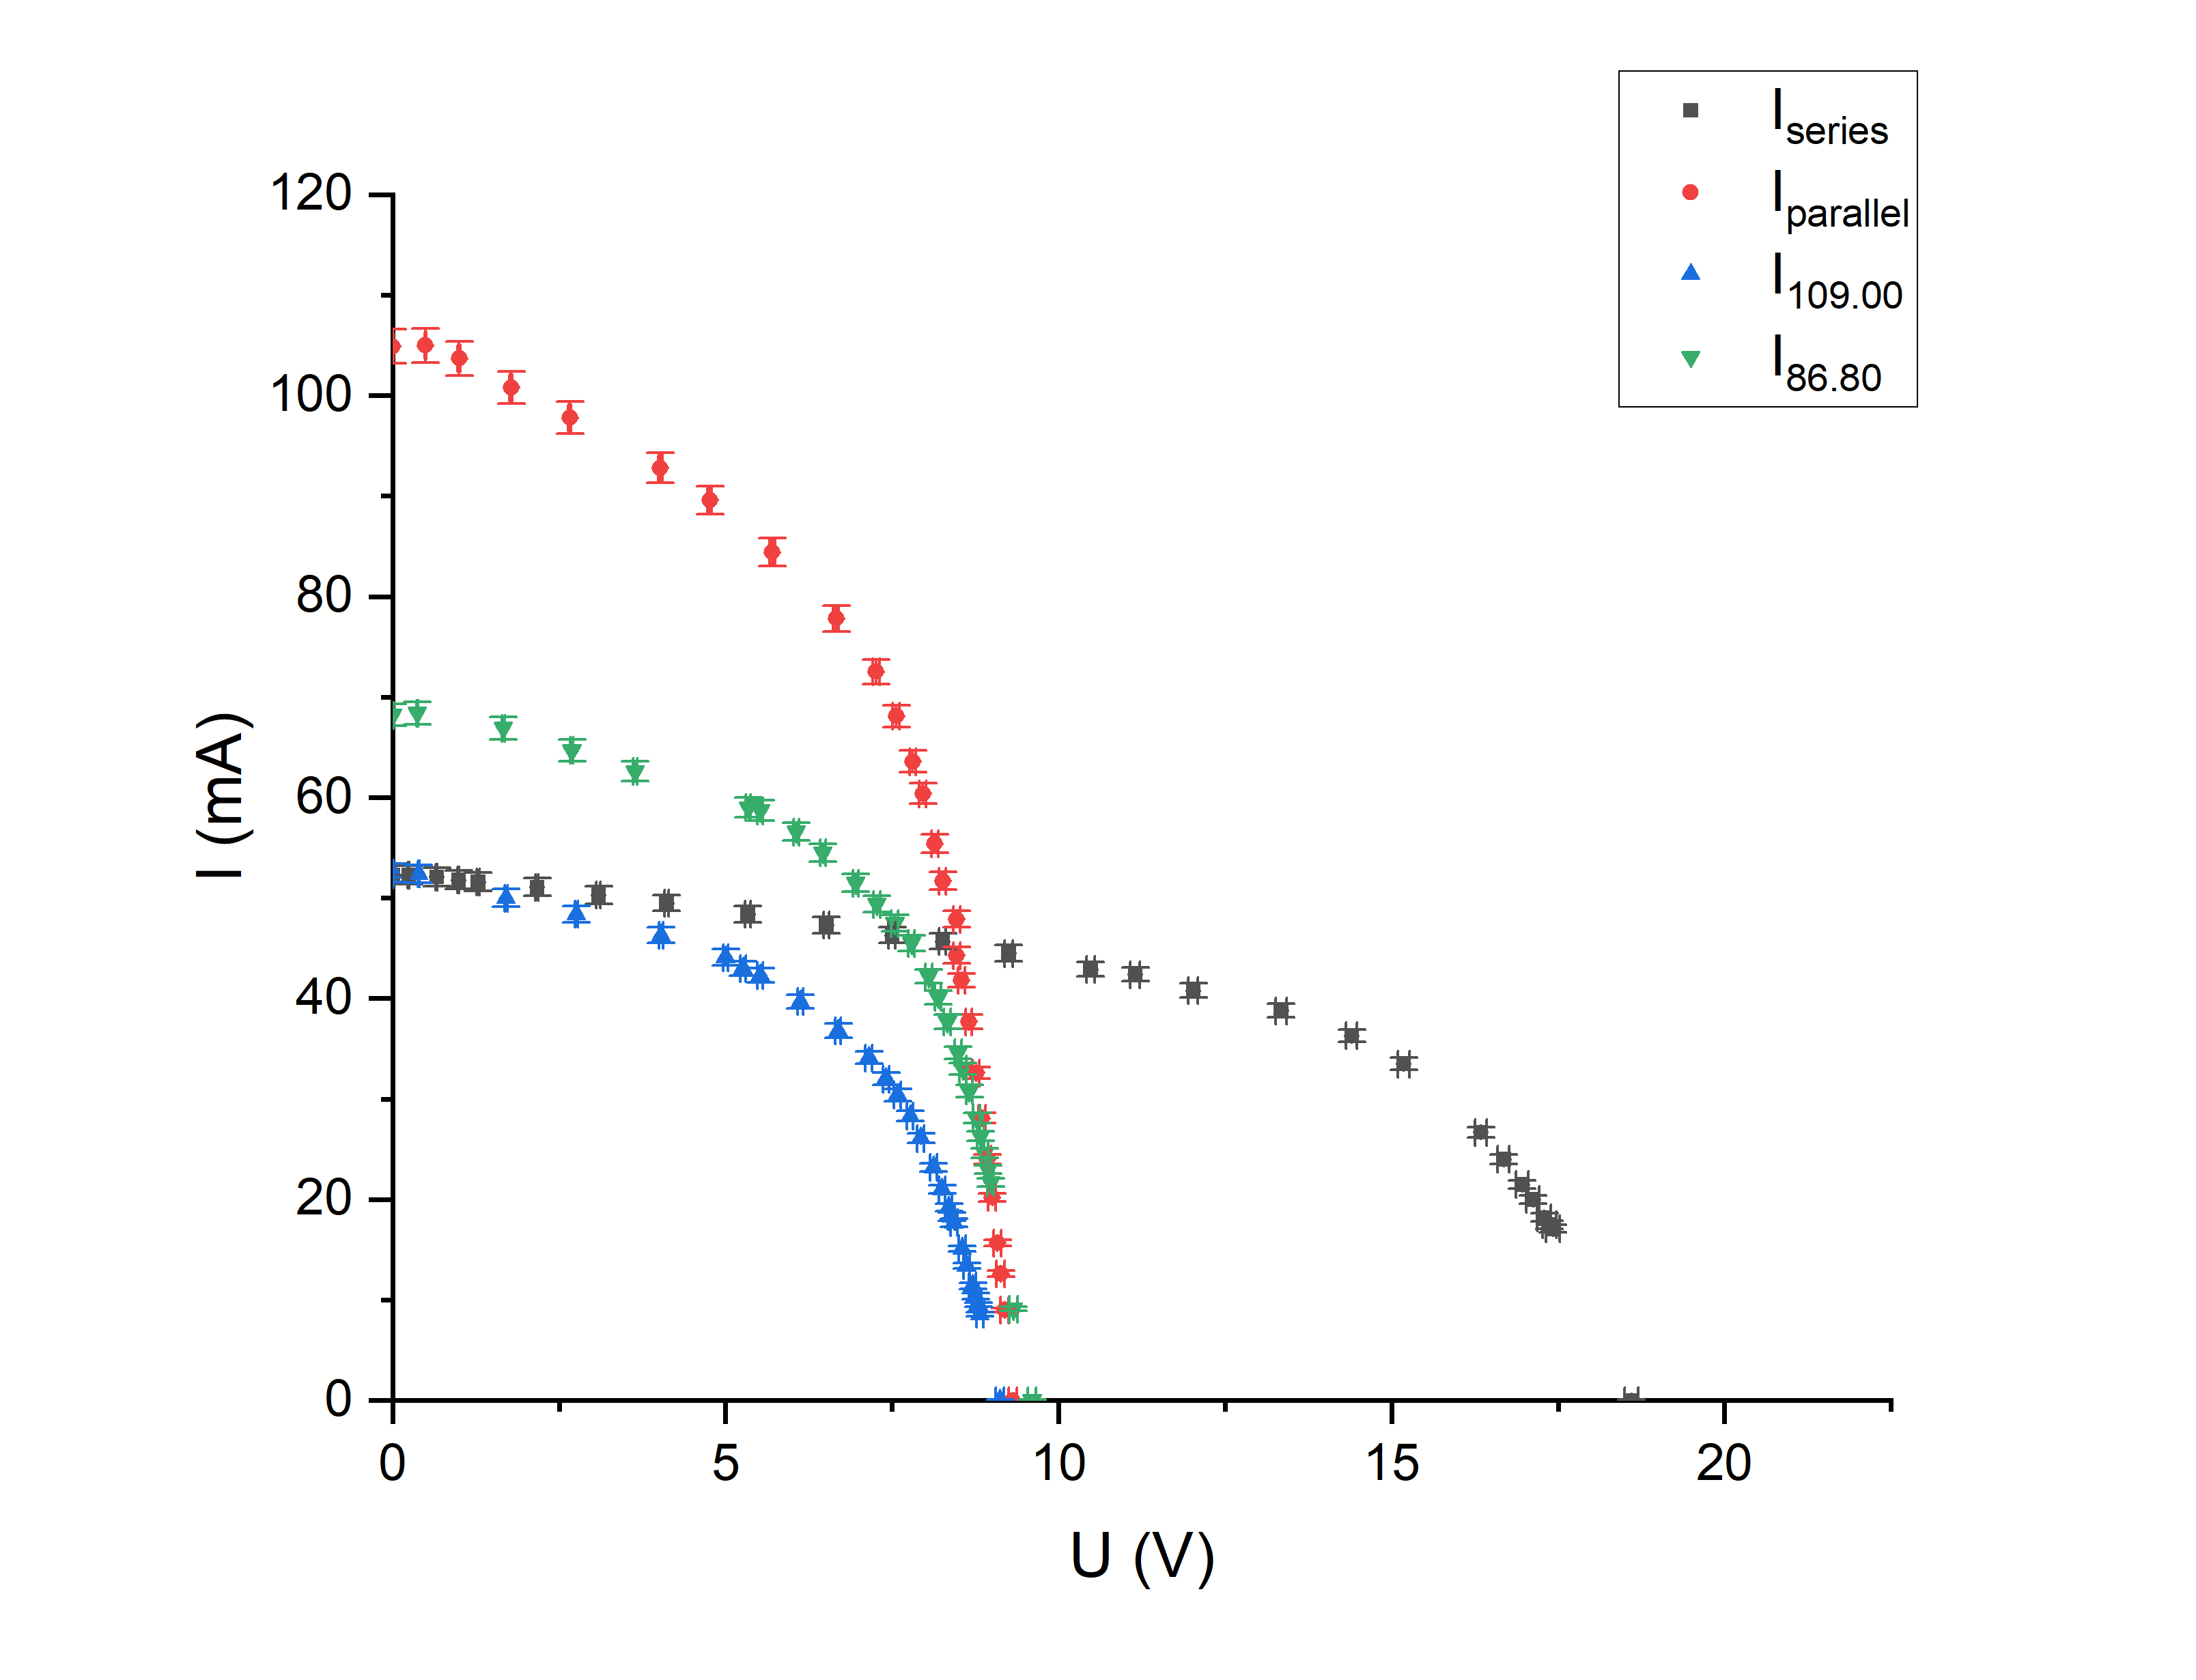
\includegraphics[scale=0.6]{I-U plot}
\caption{I-U Characteristics Curves of 4 Configurations}\label{fig.I-U}
\end{figure}

\subsection{Relation Between Output Power and Voltage}

The power $P$ of the solar cell is calculated using 
$$
P=I\cdot U.
$$
Take the first set of data (Table \ref{tab.s-p}, series) as an example,
$$P = U\cdot I = 0.24 \times 52.3 \times 10^{-3} = 0.0126 \pm 0.0004\,\,\text{W}.$$

The resistance of the external load are caluclated through Ohm's law 
$$\displaystyle R = \frac{U}{I}$$. 
Take the first set of data (Table \ref{tab.s-p}, series) as an example,
$$R = \frac{U}{I} = \frac{0.24}{52.3\times 10^{-3}} = 4.6 \pm 0.4\,\,\Omega.$$

The data are presented in Table \ref{tab.P&R}.

The characteristics curves of $P-U$ and $P-R$ are shown in Figure \ref{fig.P-U} and Figure \ref{fig.P-R}.


\begin{table}[H]
\centering
\begin{tabular}{@{}c|cc|cc||cc|cc@{}}
\toprule
 \multicolumn{1}{l}{}  & \multicolumn{4}{c||}{Series}                       & \multicolumn{4}{c}{Parallel}                    \\ \midrule
 \multicolumn{1}{l}{}  & P [W]  & $u_P$ [W] & R [$\Omega$] & $u_R$ [$\Omega$] & P [W] & $u_P$ [W] & R [$\Omega$] & $u_R$ [$\Omega$] \\ \midrule
1  & 0.0126 & 0.0006  & 4.6          & 0.4            & 0.083 & 0.002   & 1021         & 8              \\
2  & 0.0344 & 0.0009  & 12.7         & 0.5            & 0.115 & 0.003   & 725          & 6              \\
3  & 0.0513 & 0.0012  & 19.1         & 0.6            & 0.143 & 0.003   & 578          & 5              \\
4  & 0.0660 & 0.0014  & 24.8         & 0.7            & 0.182 & 0.004   & 446          & 4              \\
5  & 0.111  & 0.002   & 42.5         & 0.9            & 0.214 & 0.004   & 372          & 4              \\
6  & 0.155  & 0.003   & 61.4         & 1.1            & 0.249 & 0.005   & 315          & 3              \\
7  & 0.203  & 0.004   & 83.0         & 1.3            & 0.286 & 0.005   & 269          & 3              \\
8  & 0.258  & 0.005   & 110          & 2              & 0.357 & 0.007   & 204          & 2              \\
9  & 0.308  & 0.006   & 138          & 2              & 0.375 & 0.007   & 191          & 2              \\
10 & 0.347  & 0.006   & 162          & 2              & 0.406 & 0.007   & 177          & 2              \\
11 & 0.377  & 0.007   & 181          & 2              & 0.427 & 0.008   & 160          & 2              \\
12 & 0.412  & 0.008   & 208          & 2              & 0.451 & 0.008   & 147          & 2              \\
13 & 0.450  & 0.008   & 244          & 3              & 0.481 & 0.009   & 132          & 2              \\
14 & 0.490  & 0.009   & 295          & 3              & 0.497 & 0.009   & 123          & 2              \\
15 & 0.518  & 0.010   & 344          & 3              & 0.515 & 0.009   & 111          & 2              \\
16 & 0.523  & 0.010   & 397          & 3              & 0.526 & 0.009   & 100.1        & 1.4            \\
17 & 0.509  & 0.010   & 453          & 4              & 0.518 & 0.009   & 85.6         & 1.3            \\
18 & 0.436  & 0.009   & 612          & 5              & 0.481 & 0.008   & 67.5         & 1.1            \\
19 & 0.400  & 0.008   & 695          & 5              & 0.426 & 0.008   & 53.1         & 1.0            \\
20 & 0.365  & 0.007   & 789          & 6              & 0.373 & 0.007   & 43.3         & 0.9            \\
21 & 0.342  & 0.007   & 856          & 6              & 0.260 & 0.005   & 27.2         & 0.7            \\
22 & 0.315  & 0.007   & 950          & 7              & 0.179 & 0.003   & 17.7         & 0.6            \\
23 & 0.304  & 0.007   & 993          & 7              & 0.104 & 0.002   & 9.6          & 0.4            \\
24 & 0.298  & 0.006   & 1019         & 7              & 0.051 & 0.002   & 4.7          & 0.3            \\
25 & 0.473  & 0.009   & 263          & 3              & 0.326 & 0.006   & 229        & 3         \\ \bottomrule  
\end{tabular}

\begin{tabular}{@{}c|cc|cc||cc|cc@{}}
\toprule
 \multicolumn{1}{l}{}  & \multicolumn{4}{c||}{109.00 cm}                           & \multicolumn{4}{c}{86.80 cm}                         \\ \midrule
 \multicolumn{1}{l}{}  & P [W]  & $u_P$ [W] & R [$\Omega$] & $u_R$ [$\Omega$] & P [W]  & $u_P$ [W] & R [$\Omega$] & $u_R$ [$\Omega$] \\ \midrule
1  & 0.0204 & 0.0007    & 7.4          & 0.4              & 0.0253 & 0.0009    & 5.4          & 0.3              \\
2  & 0.085  & 0.002     & 34.0         & 0.8              & 0.111  & 0.002     & 24.8         & 0.7              \\
3  & 0.134  & 0.003     & 57.0         & 1.1              & 0.174  & 0.003     & 41.6         & 0.9              \\
4  & 0.187  & 0.003     & 87.0         & 1.4              & 0.228  & 0.004     & 58.1         & 1.1              \\
5  & 0.221  & 0.004     & 113          & 2                & 0.315  & 0.006     & 90.5         & 1.4              \\
6  & 0.233  & 0.004     & 130          & 2                & 0.324  & 0.006     & 94.0         & 1.4              \\
7  & 0.243  & 0.005     & 154          & 2                & 0.343  & 0.006     & 107          & 2                \\
8  & 0.246  & 0.005     & 182          & 2                & 0.352  & 0.006     & 119          & 2                \\
9  & 0.244  & 0.005     & 210          & 2                & 0.358  & 0.006     & 135          & 2                \\
10 & 0.237  & 0.005     & 232          & 3                & 0.359  & 0.007     & 147          & 2                \\
11 & 0.230  & 0.004     & 249          & 3                & 0.358  & 0.007     & 159          & 2                \\
12 & 0.220  & 0.004     & 275          & 3                & 0.354  & 0.006     & 171          & 2                \\
13 & 0.207  & 0.004     & 304          & 3                & 0.340  & 0.006     & 191          & 2                \\
14 & 0.188  & 0.004     & 350          & 3                & 0.328  & 0.006     & 204          & 2                \\
15 & 0.173  & 0.004     & 393          & 4                & 0.314  & 0.006     & 221          & 2                \\
16 & 0.160  & 0.003     & 435          & 4                & 0.294  & 0.006     & 245          & 3                \\
17 & 0.149  & 0.003     & 476          & 4                & 0.282  & 0.005     & 259          & 3                \\
18 & 0.129  & 0.003     & 566          & 5                & 0.267  & 0.005     & 281          & 3                \\
19 & 0.116  & 0.003     & 643          & 5                & 0.246  & 0.005     & 312          & 3                \\
20 & 0.099  & 0.002     & 764          & 6                & 0.232  & 0.005     & 336          & 3                \\
21 & 0.091  & 0.002     & 841          & 7                & 0.219  & 0.004     & 361          & 3                \\
22 & 0.084  & 0.002     & 925          & 7                & 0.206  & 0.004     & 389          & 4                \\
23 & 0.076  & 0.002     & 1026         & 8                & 0.195  & 0.004     & 414          & 4                \\
24 & 0.154  & 0.003     & 458          & 4                & 0.085  & 0.002     & 1024         & 8                \\
25 & 0.226  & 0.004     & 122          & 2                &        &           &              &        \\ \bottomrule         
\end{tabular}

\caption{Power $P$ and resistance $R$ for the different configurations.}\label{tab.P&R}
\end{table}


\begin{figure}[H]
\centering
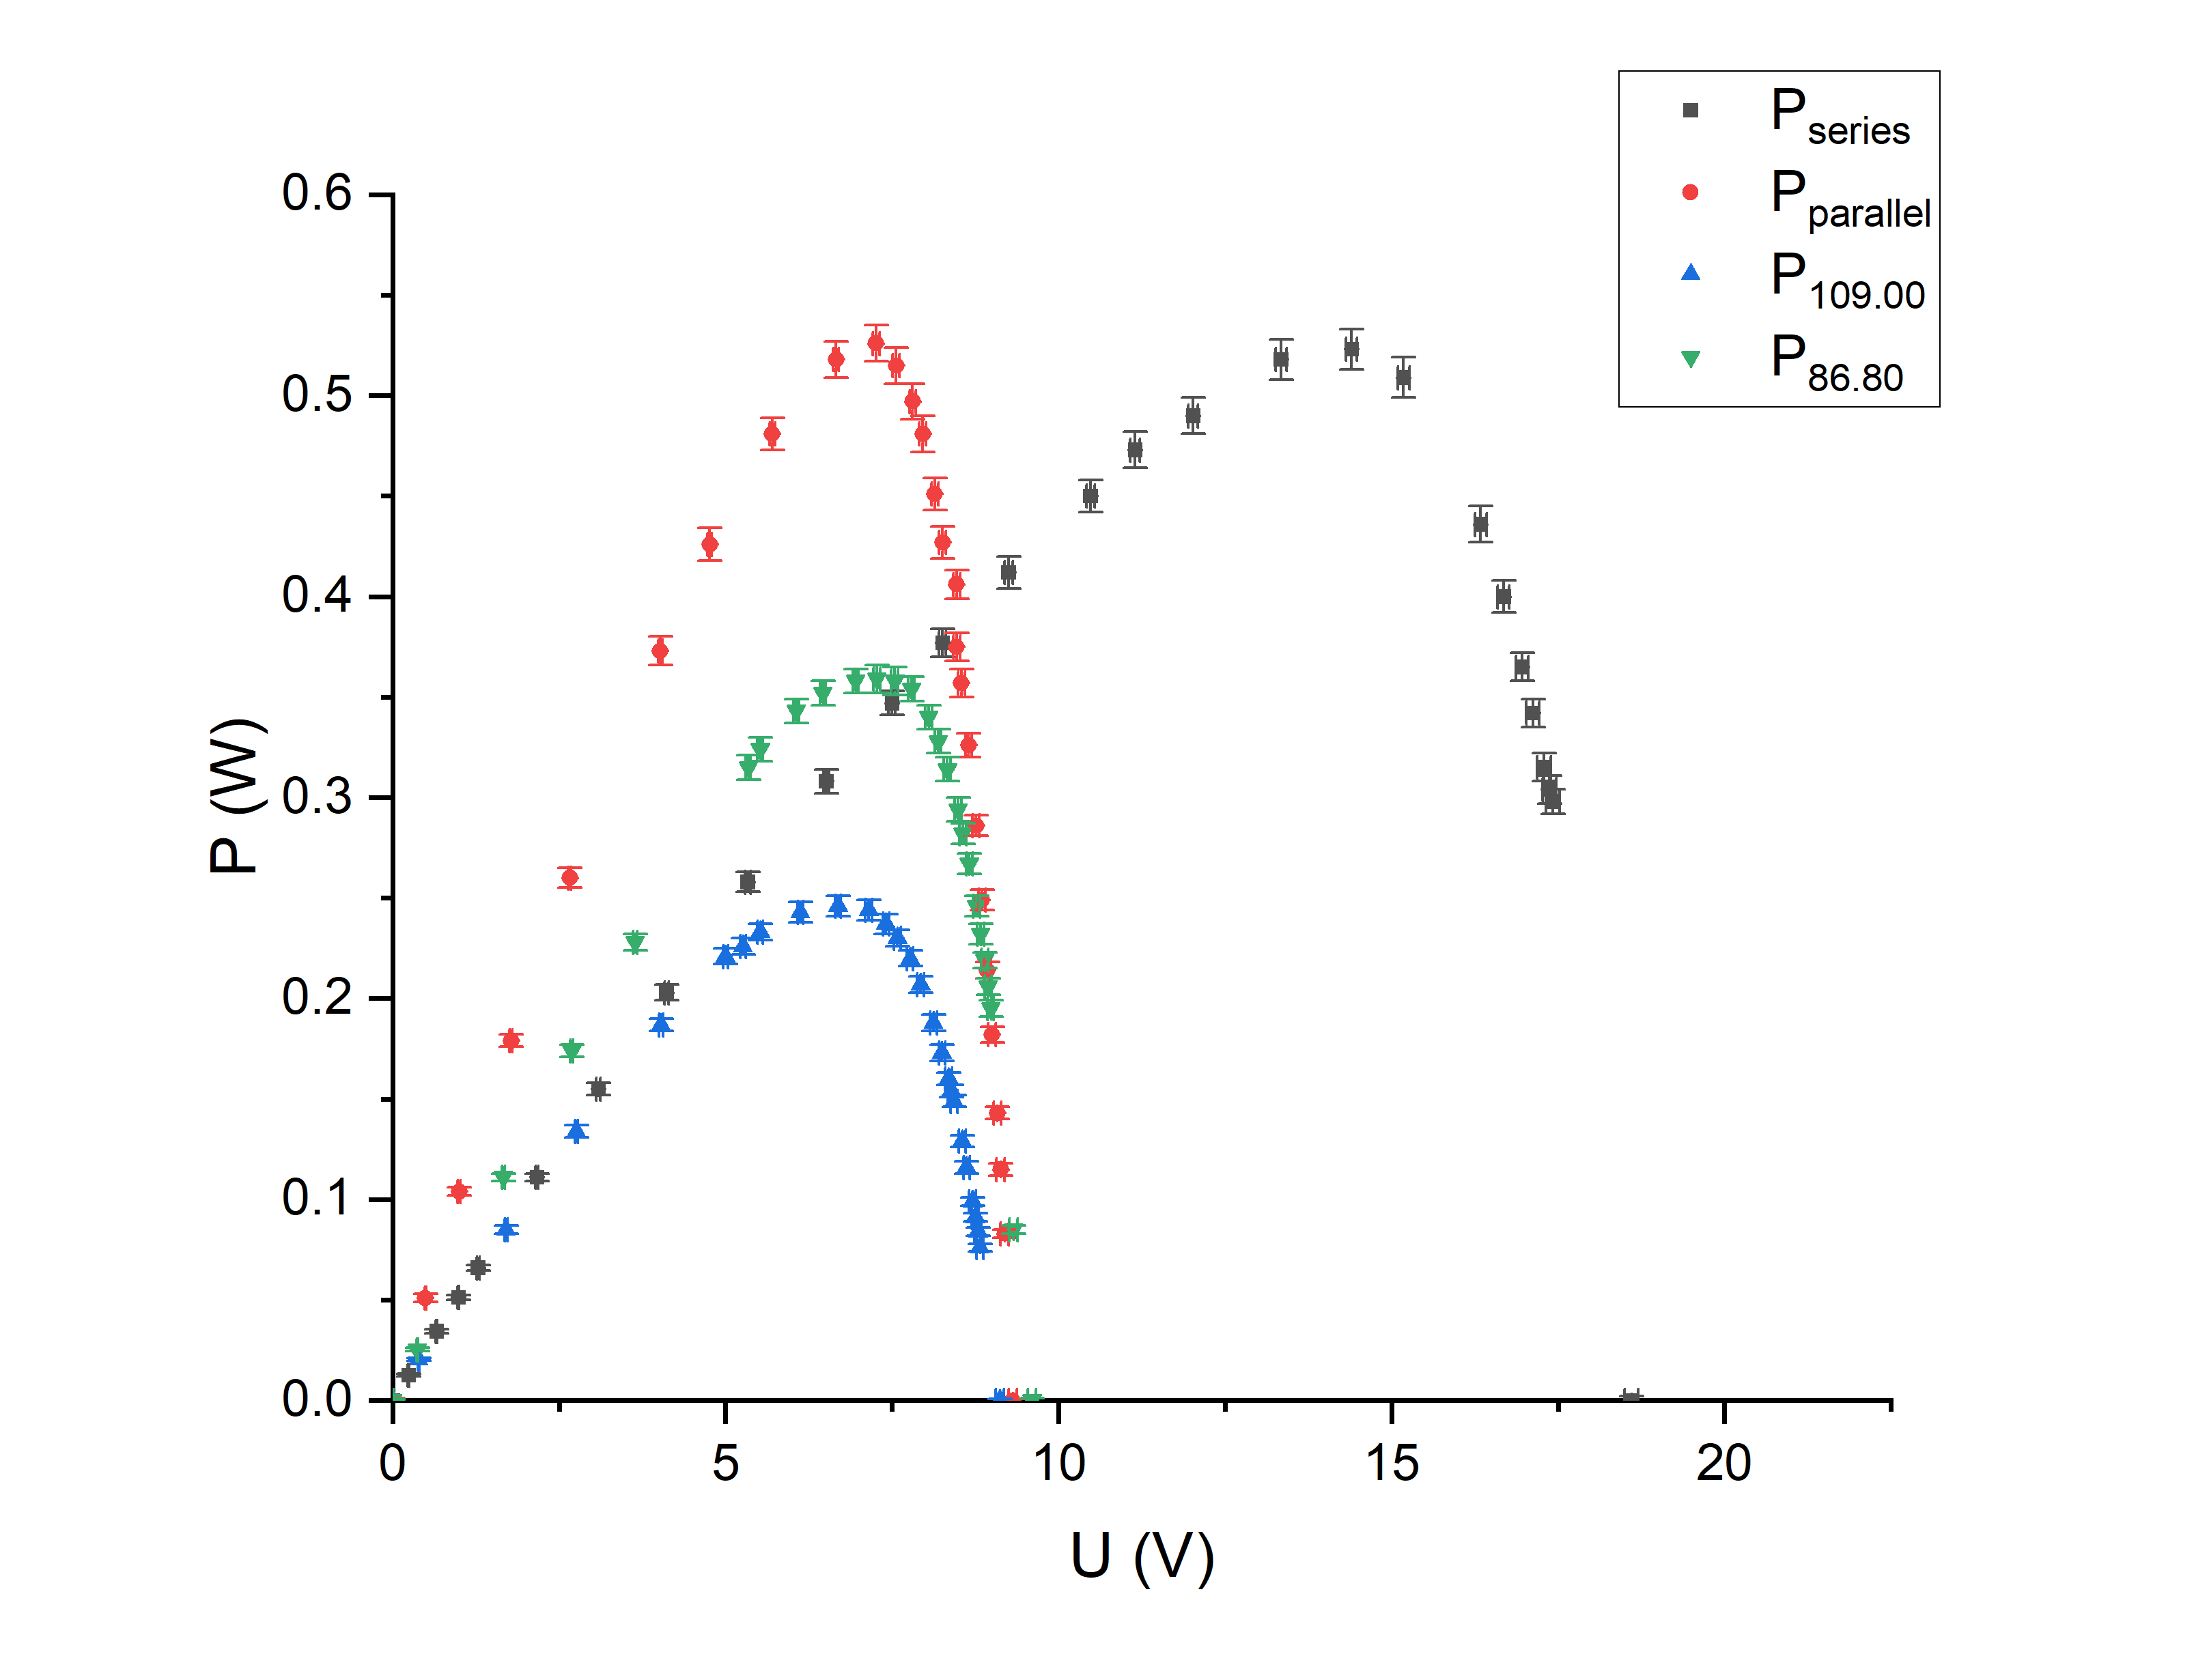
\includegraphics[scale=0.5]{P-U plot}\caption{$P$-$U$ characteristic curves of each configuration.}\label{fig.P-U}
\end{figure}

\begin{figure}[H]
\centering
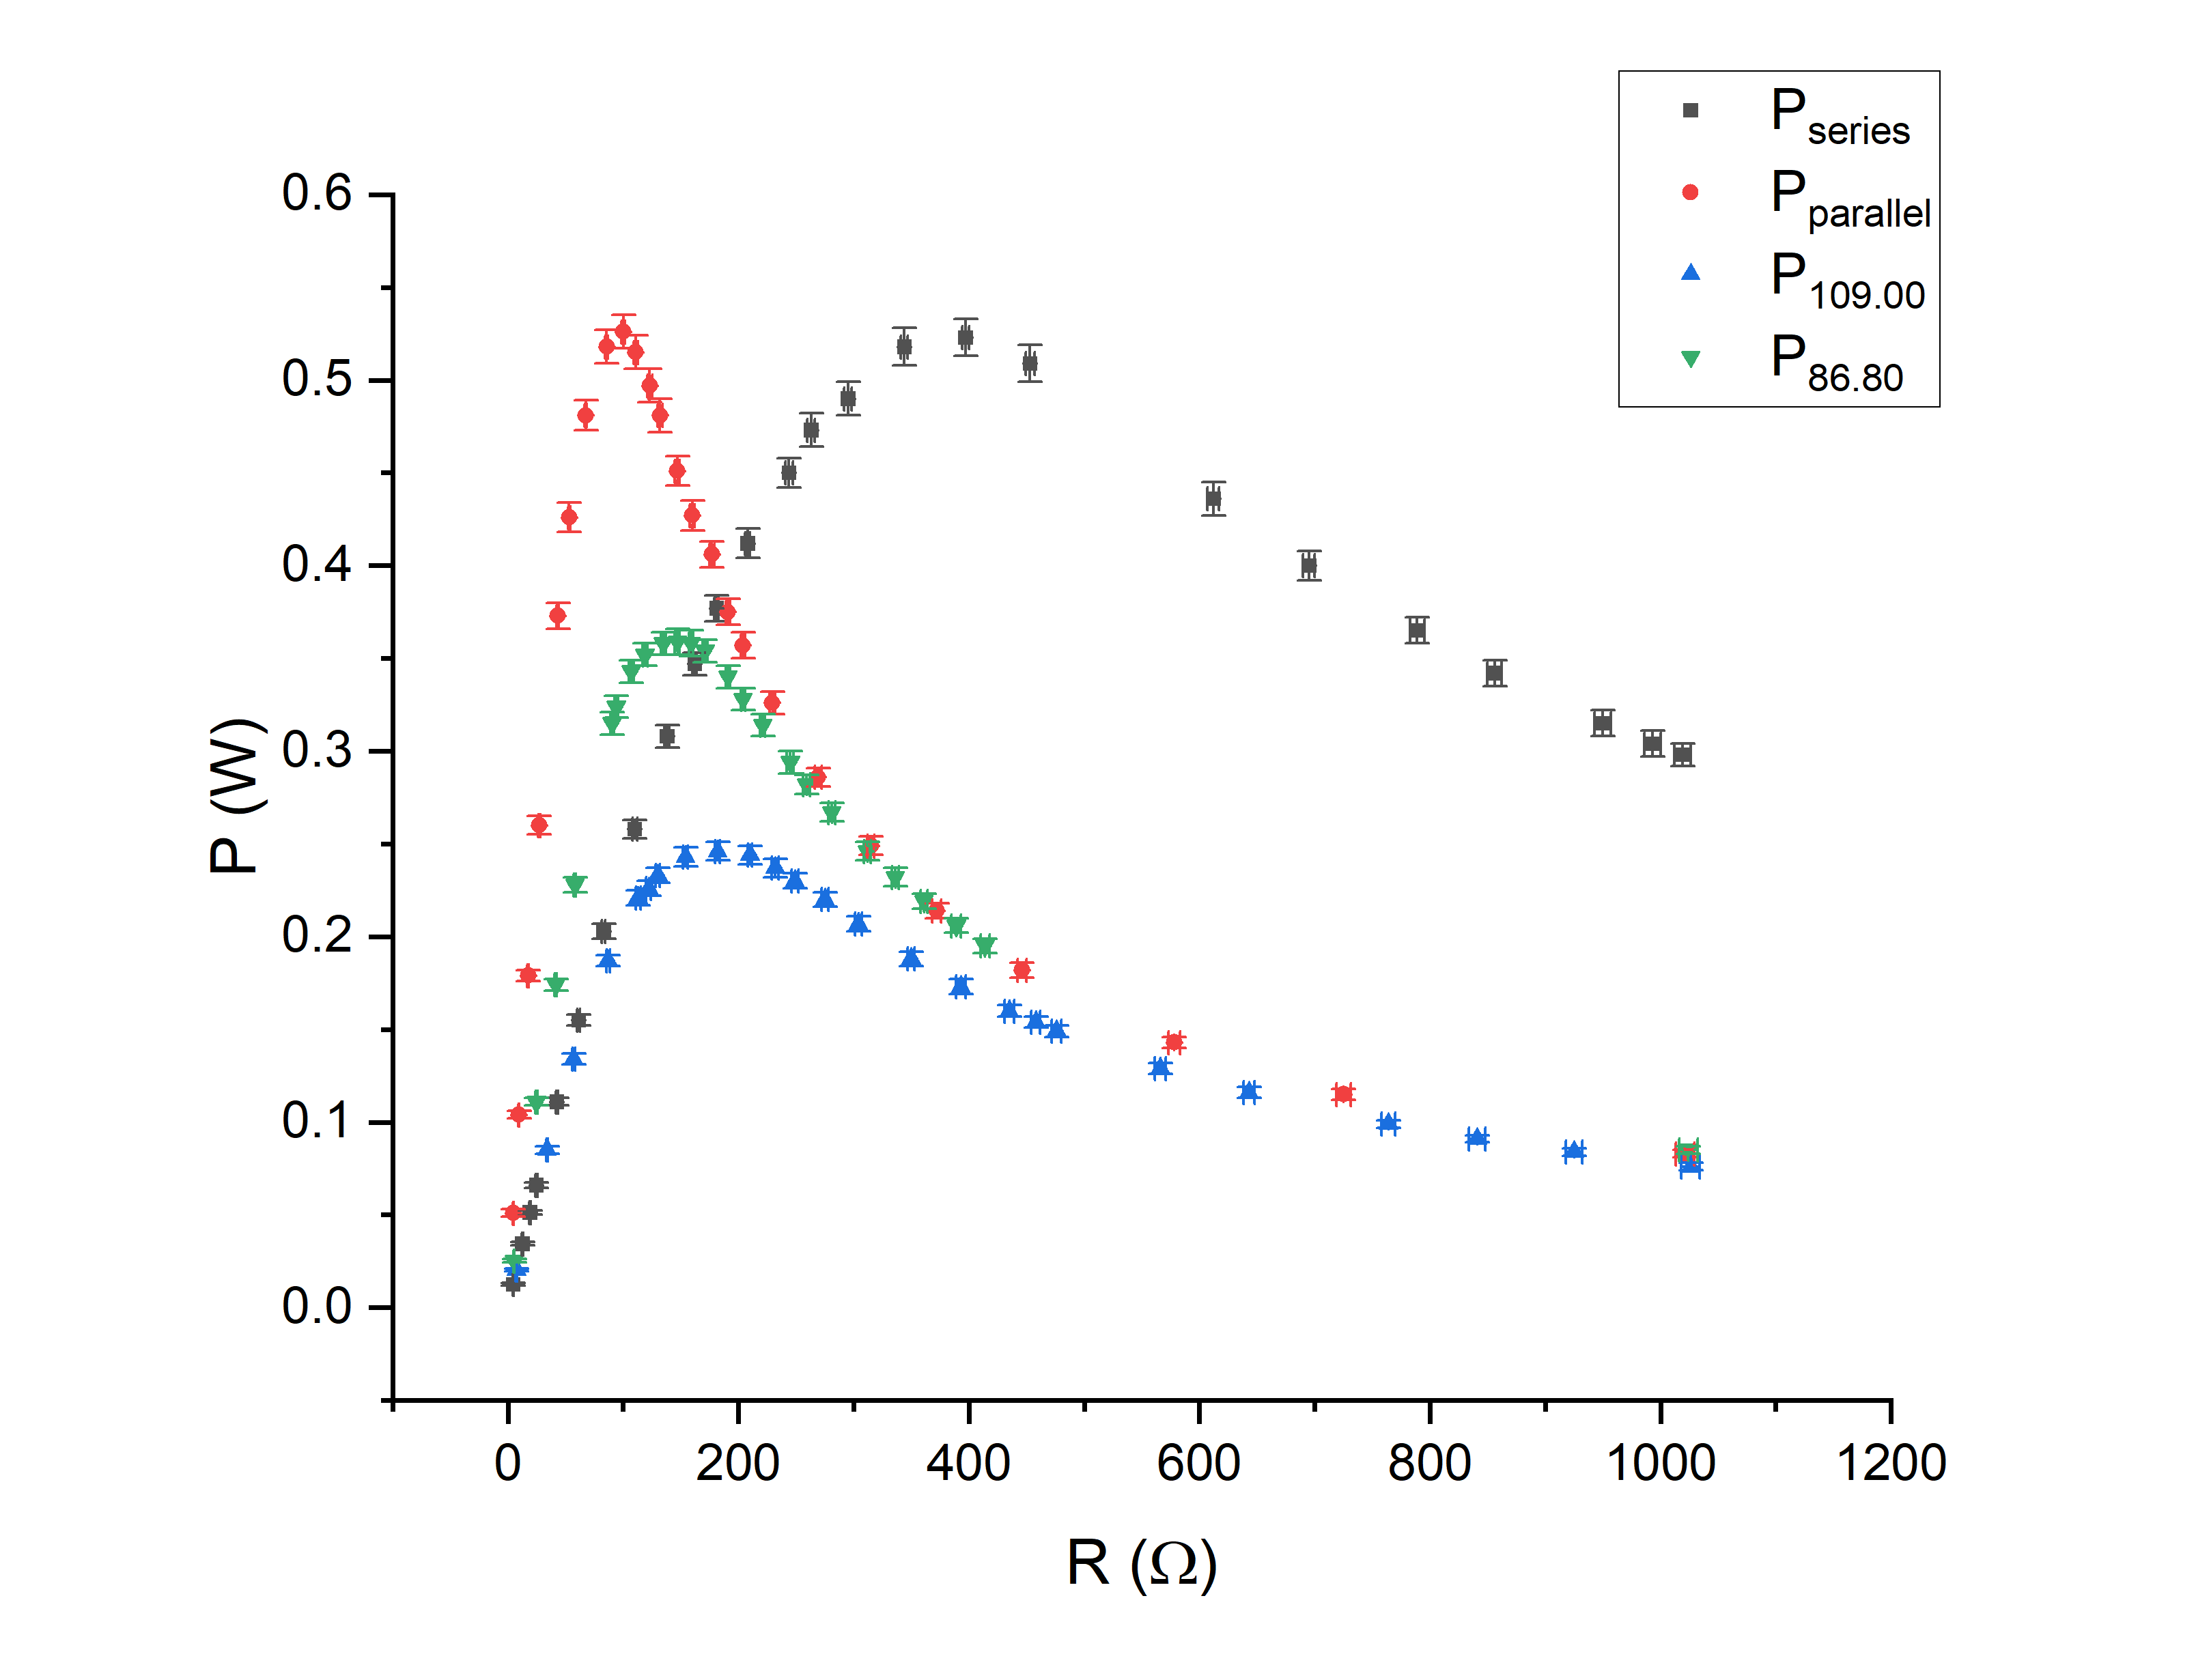
\includegraphics[scale=0.5]{P-R plot}\caption{$P$-$R$ characteristic curves of each configuration.}\label{fig.P-R}
\end{figure}

\subsection{Maximum Output Power}
According to Table \ref{tab.P&R}, when the output powers of different configurations maximize, the corresponding $I_m, V_m, R_m$ are compiled in the table below. 

\begin{table}[H]\centering
    \begin{tabular}{ccccc}
        \toprule
                 & $P_\text{m}$ [W] & $V_\text{m}$ [V] & $I_\text{m}$ [mA]   & $R_\text{m}\,\,[\Omega]$ \\
        \midrule
        Series   & 0.523 $\pm$ 0.010 & 14.40 $\pm$ 0.08    & 36.3  $\pm$ 0.6 & 397   $\pm$ 3            \\
        Parallel & 0.526  $\pm$ 0.009 & 7.26 $\pm$ 0.05    & 72.5  $\pm$ 1.2 & 100.1 $\pm$ 1.4          \\
        109.00 cm &  0.246 $\pm$ 0.005 & 6.69 $\pm$ 0.04    & 36.8  $\pm$ 0.7 & 182   $\pm$ 2            \\
        86.80 cm & 0.359  $\pm$ 0.007 & 7.27 $\pm$ 0.05    & 49.4  $\pm$ 0.8 & 147   $\pm$ 2            \\
        \bottomrule
    \end{tabular}
    \caption{$V_\text{m}$, $I_\text{m}$ and $P_\text{m}$ in each configuration.}\label{tab.Pmax}
\end{table}

\subsection{Fill Factor}

According to the definition of fill factor, it can be calculated as
$$
FF = \frac{P_{\mathrm{m}}}{I_{\mathrm{SC}}U_{\mathrm{OC}}}
$$

Therefore, take the series configuration as an example, the fill factor $FF_{\mathrm{Series}}$ can be calculated as
$$
FF_{\mathrm{Series}}=\frac{P_{\mathrm{m}}}{I_{\mathrm{SC}}U_{\mathrm{OC}}}=\frac{0.523}{18.60\times52.3\times10^{-3}}=0.538~\pm 0.015 
$$

The rest of the data are presented in Table \ref{tab.FF}.

\begin{table}[H]
\centering
\begin{tabular}{ccc}
\toprule
Configuration & $FF$ & $u_{FF}$ \\ 
\midrule
Series & 0.538 & 0.015 \\
Parallel & 0.539 & 0.015 \\
109.00 cm & 0.514 & 0.010 \\
86.80 cm & 0.555 & 0.018 \\ 
\bottomrule
\end{tabular}
\caption{Fill factors for different configurations.}\label{tab.FF}
\end{table}

\subsection{Energy Conversion Efficiency}

The measurement data are shown in Table \ref{TableArea} and Table \ref{tab.Pin}.
\begin{table}[H]\centering
    \begin{tabular}{cc}
        \toprule
        Length $L_1$ [cm] $\pm$ 0.1 [cm] & Width $L_2$ [cm] $\pm$ 0.1 [cm] \\
        \midrule
        26.00                             & 21.00                            \\
        \bottomrule
    \end{tabular}
    \caption{Measurement data for area.}\label{TableArea}
\end{table}

\begin{table}[H]\centering
    \begin{tabular}{ccccccc}
        \toprule
                                                               & 1     & 2     & 3   & 4   & 5     & 6     \\
        \midrule
        $P_{109.00}\,\,[\text{W/m}^2] \pm 10\,\,[\text{W/m}^2]$ & 388 & 332 & 217 & 174 & 152 & 129 \\
        $P_{86.80}\,\,[\text{W/m}^2] \pm 10\,\,[\text{W/m}^2]$ & 686 & 550 & 294 & 190 & 175 & 287   \\
        \bottomrule
    \end{tabular}
    \caption{Measurement data for solar power.}\label{tab.Pin}
\end{table}

Therefore,the average power per square meter can be calculated as
$$\overline{P_{109.00}} = \frac{1}{6}(388+332+217+174+152+129) = (232.0\,\pm 1.3\times10^1)\,\text{W/m}^2,$$
$$\overline{P_{86.80}} = \frac{1}{6}(686+550+294+190+175+287) = (363.7\,\pm 2.2\times 10^1)\,\text{W/m}^2.$$

Then the total power is
$$P_{\text{in},109.00} = \overline{P_{109.00}}L_1L_2 = 232 \times 0.260 \times 0.210 = 12.7 \pm 0.9\,\,\text{W},$$
$$P_{\text{in},86.80} = \overline{P_{86.80}}L_1L_2 = 363.7 \times 0.260 \times 0.210 = 19.9\pm 1.5\,\,\text{W}.$$

The power energy conversion efficiency $\eta$ can be calculated as
$$\eta_{109.00} = \frac{P_\text{m}}{P_{\text{in},109.00}} \times 100\% = \frac{0.246}{12.7} \times 100\%= 1.9\% \pm 0.2\%,$$
$$\eta_{86.80} = \frac{P_\text{m}}{P_{\text{in},86.80}} \times 100\% = \frac{0.359}{19.9} \times 100\%= 1.8\% \pm 0.2\%,$$

\section{Conclusion and Discussion}

\subsection{I-V Relation}
In this part, the relation between the current $I$ and the voltage $V$ is studied.  From Figure \ref{fig.I-U}, it can be seen that generally, as voltage $V$ increases, current $I$ decreases. And the rate of change of current $I$ also increases as voltage $V$ increases. Comparing the curves of \textbf{series} and \textbf{parallel} configurations, it can be seen that the open circuit voltage $U_{OC}$ doubled as the circuit changes from parallel configuration to series configuration, while the short circuit current $I_{SC}$ halved. This trend fits with the characteristics of series and parallel circuit.
\subsection{P-V and P-R Relation, and Maximum Power Output}
For the $P-V$ relation, from Figure \ref{fig.P-U},it can be summarized that as the voltage $U$ increases, the power $P$ first increases from 0, reaching a peak, and then decreases to zero again. 

As for thr $P-R$ relation, from Figure \ref{fig.P-R}, it is obvious that, similarly,  as the voltage $U$ increases, the power $P$ first increases from 0, reaching a peak, and then decreases to zero again.  Furthermore,the output power attains its maximum at approximately $R = R_m$.  The curves fit with the result in section 3.3 about maximum power output, verifying both results.
\subsection{Fill Factor and Energy Conversion Efficiency}
The fill factors and energy conversion efficiencies of two groups of result of different distances don't differentiate much from each other. However, according to the lab manual \cite{manual}, theoretically speaking, the greater the fill factor, the greater the energy conversion efficiency should be, which is no the case in this lab. This will be discussed in the later part.

One conclusion can be derived is that the closer the solar board is to the light source, the greater the incident intensity, the greater the fill factor will be. This agree with out common sense and theory.

The experimental results of energy conversion efficiency are 1.9\% and 1.8\%. Notice that the energy conversion efficiency of the solar board is very low, which can explain that in real life, the solar panels are often of big area and large number, which compensates the defect in low energy conversion efficiency.

\subsection{Discussion and Suggestion}
There are several factors that might cause errors in this experiment:

\begin{enumerate}
\item The light source used in the lab is highly non-uniform, which means there may exist huge difference in the distribution of light on the solar board. Therefore the average power absorbed by the solar board may be inaccurate, causing errors in the calculation of energy conversion efficiency.
\item About the determination of the maximum power output and corresponding parameters, as only discrete data points are obtained and no fitting is performed, the values of $V_m, I_m, R_m$ of maximum power output might be inaccurate, which are only selected from the existing data points.
\item In the experiment, the solar board is viewed to be ideal and with no resistance. However, there are actually considerable inner resistance, causing errors in determining the $P-R$ relation.
\end{enumerate}

Some possible improvements can be made to the experiment:
\begin{enumerate}
\item Measure more data for the power per square meter on the solar board;
\item Perform fitting to correct the $P-R$ and $P-V$ curves, then obtain the corresponding parameters of maximum power output from the fitting curves;
\item Measure the inner resistance of the solar board and subtract when calculating the outer resistance.
\end{enumerate}


\begin{thebibliography}{10}
	\bibitem{manual} VP241 Exercise 3: Solar Cells: $I$-$V$ Characteristics, UM-SJTU Joint Institude.
\end{thebibliography}

\newpage

\begin{appendix}

\section{Uncertainty Analysis}

\subsection{I-V Relation}
The uncertainty of $V$ is $\pm(0.5\%+0.01)$ V, and the uncertainty of $I$ is $\pm(1.5\%+0.1)$ mA. 

For uncertainty calculation, take the first set of data as an example,
$$u_{V} = 0.5\% \times 0.24 + 0.01 = 0.011\,\text{V}.$$
$$u_{I} = 1.5\% \times 52.3 + 0.1 = 0.9\,\text{mA}.$$
All the uncertainties of $V$ and $I$ are calculated in this way and the results are shown in Table \ref{tab.UncIV}.

\begin{table}[H]\centering
    \begin{tabular}{c|cc||cc||cc||cc}
        \toprule
   & \multicolumn{2}{c||}{\textbf{Series}} & \multicolumn{2}{c||}{\textbf{Parallel}} & \multicolumn{2}{c||}{\textbf{109.00 cm}} & \multicolumn{2}{c}{\textbf{86.80 cm}} \\
        \midrule
           & $u_V$ [V]                    & $u_I$ [mA]                     & $u_V$ [V]                      & $u_I$ [mA]                   & $u_V$ [V] & $u_I$ [mA] & $u_V$ [V] & $u_I$ [mA] \\
        \midrule
1  & 0.011            & 0.9              & 0.06              & 0.2               & 0.012              & 0.9               & 0.01              & 1.1               \\
2  & 0.013            & 0.9              & 0.06              & 0.3               & 0.02               & 0.9               & 0.02              & 1.1               \\
3  & 0.015            & 0.9              & 0.06              & 0.3               & 0.02               & 0.8               & 0.02              & 1.1               \\
4  & 0.02             & 0.9              & 0.06              & 0.4               & 0.03               & 0.8               & 0.03              & 1.0               \\
5  & 0.02             & 0.9              & 0.05              & 0.5               & 0.04               & 0.8               & 0.04              & 1.0               \\
6  & 0.03             & 0.9              & 0.05              & 0.5               & 0.04               & 0.7               & 0.04              & 1.0               \\
7  & 0.03             & 0.8              & 0.05              & 0.6               & 0.04               & 0.7               & 0.04              & 0.9               \\
8  & 0.04             & 0.8              & 0.05              & 0.7               & 0.04               & 0.7               & 0.04              & 0.9               \\
9  & 0.04             & 0.8              & 0.05              & 0.8               & 0.05               & 0.6               & 0.04              & 0.9               \\
10 & 0.05             & 0.8              & 0.05              & 0.8               & 0.05               & 0.6               & 0.05              & 0.8               \\
11 & 0.05             & 0.8              & 0.05              & 0.9               & 0.05               & 0.6               & 0.05              & 0.8               \\
12 & 0.06             & 0.8              & 0.05              & 0.9               & 0.05               & 0.5               & 0.05              & 0.8               \\
13 & 0.06             & 0.7              & 0.05              & 1.0               & 0.05               & 0.5               & 0.05              & 0.7               \\
14 & 0.07             & 0.7              & 0.05              & 1.1               & 0.05               & 0.4               & 0.05              & 0.7               \\
15 & 0.08             & 0.7              & 0.05              & 1.1               & 0.05               & 0.4               & 0.05              & 0.7               \\
16 & 0.08             & 0.6              & 0.05              & 1.2               & 0.05               & 0.4               & 0.05              & 0.6               \\
17 & 0.09             & 0.6              & 0.04              & 1.3               & 0.05               & 0.4               & 0.05              & 0.6               \\
18 & 0.09             & 0.5              & 0.04              & 1.4               & 0.05               & 0.3               & 0.05              & 0.6               \\
19 & 0.09             & 0.5              & 0.03              & 1.4               & 0.05               & 0.3               & 0.05              & 0.5               \\
20 & 0.09             & 0.4              & 0.03              & 1.5               & 0.05               & 0.3               & 0.05              & 0.5               \\
21 & 0.10             & 0.4              & 0.02              & 1.6               & 0.05               & 0.3               & 0.05              & 0.5               \\
22 & 0.10             & 0.4              & 0.02              & 1.6               & 0.05               & 0.2               & 0.05              & 0.4               \\
23 & 0.10             & 0.4              & 0.02              & 1.7               & 0.05               & 0.2               & 0.05              & 0.4               \\
24 & 0.10             & 0.4              & 0.012             & 1.7               & 0.05               & 0.4               & 0.06              & 0.2               \\
25 & 0.07             & 0.7              & 0.05              & 0.7               & 0.04               & 0.7               &                   &                    \\
        \bottomrule
    \end{tabular}
    \caption{Uncertainty of the data for $I$-$V$ characteristic.}\label{tab.UncIV}
\end{table}

\subsection{P-V and P-R Relation}

For $P = VI$, its uncertainty is calculated as
$$u_P = \sqrt{(\frac{\partial P}{\partial V}u_V)^2 + (\frac{\partial P}{\partial I}u_I)^2} = \sqrt{(Iu_V)^2 + (Vu_I)^2}.$$

For $R = \frac{V}{I}$, its uncertainty is calculated as
$$u_R = \sqrt{(\frac{\partial R}{\partial V}u_V)^2 + (\frac{\partial R}{\partial I}u_I)^2} = \sqrt{(\frac{u_V}{I})^2 + (-\frac{V}{I^2}u_I)^2}.$$

Take the first set of data as an example,
$$u_P = \sqrt{(Iu_V)^2 + (Vu_I)^2} = \sqrt{(52.3\times 10^{-3}\times 0.011)^2 + (0.24\times 0.9\times 10^{-3})^2} = 0.0006\,\text{W}.$$
$$u_R = \sqrt{(\frac{u_V}{I})^2 + (-\frac{V}{I^2}u_I)^2} = \sqrt{(\frac{0.01}{52.3\times 10^{-3}})^2 + (-\frac{0.24}{(52.3\times10^{-3})^2}\times 0.9)^2} = 0.4\,\Omega .$$

The uncertainty of $P$ and $R$ of all data are calculated in this way and the results are shown in Table \ref{tab.P&R} in the \textbf{Result} part, following the values of $P$ and $R$.

\subsection{Fill Factor}
The uncertainty of $V_\text{oc}$ and $I_\text{sc}$ is calculated in the same way as $V$ and $I$ in the previous part. The results are shown below.

\begin{table}[H]\centering
    \begin{tabular}{cccc}
        \toprule
                 & $u_{V_\text{oc}}$ [V] & $u_{I_\text{sc}}$ [mA] & $u_{P_\text{m}}$ [W] \\
        \midrule
        Series & 0.10 & 0.9 & 0.010 \\
        Parallel & 0.06 & 1.7 & 0.009 \\
        109.00 cm & 0.06 & 0.9 & 0.005 \\
        86.80 cm & 0.06 & 1.1 & 0.007 \\
        \bottomrule
    \end{tabular}
    \caption{Uncertainty of $V_\text{oc}$ and $I_\text{sc}$.}
    \label{tab:uncocsc}
\end{table}

The uncertainty of fill factor, $FF = P_\text{m}/(V_\text{oc}I_\text{sc})$, is calculated as
\begin{align*}
    u_{FF} & = \sqrt{(\frac{\partial FF}{\partial P_\text{m}}u_{P_\text{m}})^2 + (\frac{\partial FF}{\partial V_\text{oc}}u_{V_\text{oc}})^2 + (\frac{\partial FF}{\partial I_\text{sc}}u_{I_\text{sc}})^2}   \\
           & = \sqrt{(\frac{1}{V_\text{oc}I_\text{sc}}u_{P_\text{m}})^2 + (-\frac{P_\text{m}}{V_\text{oc}^2I_\text{sc}}u_{V_\text{oc}})^2 + (-\frac{P_\text{m}}{V_\text{oc}I_\text{sc}^2}u_{I_\text{sc}})^2},
\end{align*}

Take the first set of data as an example,
\begin{align*}
    u_{FF} & = \sqrt{(\frac{1}{V_\text{oc}I_\text{sc}}u_{P_\text{m}})^2 + (-\frac{P_\text{m}}{V_\text{oc}^2I_\text{sc}}u_{V_\text{oc}})^2 + (-\frac{P_\text{m}}{V_\text{oc}I_\text{sc}^2}u_{I_\text{sc}})^2}      \\
           & = \sqrt{(\frac{1}{18.6\times 52.3\times 10^{-3}}\times 0.010)^2 + (-\frac{0.523}{18.60^2\times 52.3\times 10^{-3}}\times 0.010)^2 + (-\frac{0.523}{18.60\times (52.3\times 10^{-3})^2}\times 0.0009)^2} \\
           & = 0.015.
\end{align*}

The uncertainties are calculated as shown above and the rest of the results are shown in Table \ref{tab.FF} in the \textbf{Result} part.

\subsection{Energy Conversion Efficiency }
In this part, as multiple measurements are performed, both type-A and type-B uncertainty need to be considered. The type--$B$ uncertainty of power measurement is $u_{P} = \Delta_{P,B} = \Delta_{dev} = 10\,\,[\text{W/m}^2]$. 

Since the power measurement is carried for 6 times, the type--$A$ is
\begin{align*}
    \Delta_{P,A}
    =    & \frac{2.57}{\sqrt{6}}\sqrt{\frac{1}{6-1}\sum \limits_{i=1}^{6}(P_i-\overline{P})^2}.
\end{align*}

The total uncertainty is then
$$u_{\overline{P}} = \sqrt{\Delta_{P,A}^2+\Delta_{P,B}^2} = \sqrt{\bigg(\frac{2.57}{\sqrt{6}}\sqrt{\frac{1}{6-1}\sum \limits_{i=1}^{6}(P_i-\overline{P})^2}\bigg)^2+10^2}.$$

Hence, for the two single configurations,
$$u_{\overline{P_{109.00}}} = \sqrt{\bigg(\frac{2.57}{\sqrt{6}}\sqrt{\frac{1}{6-1}\sum \limits_{i=1}^{6}(P_i-232.0)^2}\bigg)^2+10^2} = 1.3\times 10^1\,\,\text{W/m}^2,$$
$$u_{\overline{P_{86.80}}} = \sqrt{\bigg(\frac{2.57}{\sqrt{6}}\sqrt{\frac{1}{6-1}\sum \limits_{i=1}^{6}(P_i-363.7)^2}\bigg)^2+10^2} = 2.2\times 10^1\,\,\text{W/m}^2,$$

The uncertainty of $P_\text{in} = \overline{P}L_1L_2$ is calculated as
\begin{align*}
    u_{P_\text{in}} & = \sqrt{(\frac{\partial P_{\text{in}}}{\partial \overline{P}}u_{\overline{P}})^2 + (\frac{\partial P_{\text{in}}}{\partial L_1}u_{L_1})^2 + (\frac{\partial P_\text{in}}{\partial L_2}u_{L_2})^2} \\
                    & = \sqrt{(L_1L_2u_{\overline{P}})^2 + (\overline{P}L_2u_{L_1})^2 + (\overline{P}L_1u_{L_2})^2}.
\end{align*}

Hence, plugging in the values yields that
$$u_{P_{\text{in},109.00}} = 0.9\,\,\text{W},\hspace{2em}u_{P_{\text{in},86.80}} = 1.5\,\,\text{W}.$$

Finally, the uncertainty of $\eta = \frac{P_{\text{m}}}{P_\text{in}}\times 100\%$ can be calculated as
\begin{align*}
    u_\eta & = \sqrt{(\frac{\partial \eta}{\partial P_\text{m}}u_{P_\text{m}})^2 + (\frac{\partial \eta}{\partial P_\text{in}}u_{P_\text{in}})^2} \times 100\% \\
           & = \sqrt{(\frac{1}{P_\text{in}}u_{P_\text{m}})^2 + (-\frac{P_{\text{m}}}{P_{\text{in}}^2}u_{P_\text{in}})^2} \times 100\%.
\end{align*}

Plugging in the values yields
$$u_{\eta_{109.00}} = 0.2\,\%,\hspace{2em}u_{\eta_{86.80}} = 0.2\,\%.$$

\section{Data Sheet}
The original data sheet is appended in the last part.

\end{appendix}

\end{document}